\chapter{Passive Haptics Experiment}
\label{chap:ph_exp}

\section{Introduction}

Passive haptics is a term that has been used to describe a variety of technologies or techniques to provide the sense of touch to a user of a virtual environment.
It is often defined by its distinction from active haptics, which simulate the sense of touch with energy exchange, typically electromechanical.
A common active haptic technology used in immersive virtual environments is a haptic glove, often utilizing small motors at the fingertips.
In contrast, passive haptics often utilize proxy objects placed in the physical world to co-incide with the virtual environment experience.
The proxy objects can be simple or complex.
They can be colocated and accurate with the virtual world or purposefully designed to trick the user.
In our paper, we utilize a simple colocated passive haptic device and measure its effect on the presence and performance of subjects using a 2D panel in a 3D immersive virtual environment.

The advantages to using a simple passive haptic can be easily understood: less cost and complexity compared to most active haptic solutions.
However, the disadvantage comes with its inflexibility.
Due to their nature, passive haptics often have to be purpose built for a single or limited experience.
While past research has aimed to address this, by either actively positioning a proxy object or simplifying the proxy object to fool the user, our application does not suffer from this limitation.
The motivation for our research comes from the application of designing aerospace cockpits, complex human-machine interfaces where the user is stationed at their workspace.
For the purpose of evaluating a cockpit design, the user does not need a dynamic tactile environment.
Furthermore, many cockpit design processes already create a physical mockup which can provide the passive haptics for this evaluation.

We present our findings in testing passive haptics versus no haptics in an immersive virtual reality environment.
Using a head-mounted display and a hand tracker, the subjects performed the same Fitts' Law style task under these two haptic conditions.
The passive haptics was a flat surface placed at an angle on a desk in front of their seating area.
Their performance on the Fitts' task was recorded as well as their responses to a presence survey, a self reported arm fatigue score and a general questionnaire.

\section{Background}

\subsection{Haptics}

Passive haptics has been a topic of research since the early immersive virtual environments.
Robotic passive haptics were used to ameloriate the inflexibility of a proxy object by utilizing a robotic arm to position the proxy object in the virtual environment where the user was reaching\cite{tachi_construction_1994,mcneely_robotic_1993}.
Insko\cite{insko_passive_2001} found increased presence using passive haptics for a maze, and also found that subjects trained with the passive haptics performed better after they were removed than the group that never used them.
Another track of work combined active haptics with passive haptics, using a haptic glove with a physical panel to create mixed haptics \cite{borst_evaluation_2005}.
Again, performance was increased with the haptics, but minimal differences were found between using the mixed haptics and the passive haptics alone.
Similar to our motivation and work, Schiefele et al.\cite{schiefele_simple_1998} replaced a cockpit panel with a flat panel in an immersive head-mounted virtual environment, and found that users could activate buttons and switches in less time with the panel present than without.
While much of the research involving passive haptics indicates an increase in the presence of the user, some have questioned whether active haptics provides benefits.
Pontonnier et al.\cite{pontonnier_designing_2014} discovered that subjects had decreased presence ratings in a virtual assembly task when using a haptic glove, versus both a real environment and a virtual environment without haptics.
We build on this previous work by investigating the effects of passive haptics with the lastest virtual enviroment technology, as well as performing a complete Fitts' Law characterization between no haptics and passive haptics.

\subsection{Fitts' Law}

Fitts' originally devised a relationship between movement time and the distance and size of targets for a human performing rapid aimed movements\cite{fitts_information_1954}.
This has since become known as Fitts' Law, and later work has refined the index of difficulty (${ID}$) as:
\begin{equation}
    {ID}=\log_2\left(\frac{D}{W}+1\right)
    \label{eq:index_of_difficulty}
\end{equation}
where $D$ is the distance to the target from the starting location and $W$ is the width of the target.
This formula for index of difficulty is known as the Shannons' formulation\cite{mackenzie_note_1989}.

Commonly, the index of difficulty is related to movement time (${MT}$) through a linear regression.
However, in this work we are concerned with the measurement known as throughput (${TP}$).
Throughput has been recommended as the dependent measures for comparisons between experimental conditions\cite{soukoreff_towards_2004}.
As the name suggests, it can be thought of as the rate of information the human can input with the particular experimental setup or input device.
It is defined as the index of difficulty over the movement time, and has the units of ``bits per second.''
\begin{equation}
    {TP}=\frac{ID}{MT}
    \label{eq:throughput}
\end{equation}

The use of Fitts' Law as a tool for human-computer interface research began with the research of Card et al.\cite{card_evaluation_1978} for the evaluation of different input devices for text entry.
In 2000, The ISO 9241-9 standard was published with guidance on using Fitts' Law as an evaluation of pointing devices\cite{international_organization_for_standardization_iso_2000}.
Along with the ISO standard, there have been calls to standardize the use of Fitts' Law so that results can be compared across literature\cite{soukoreff_towards_2004}.
For a 2-dimensional task (where all the buttons exist on a single plane), it is reccomended to use the circle layout as shown in Figure \ref{fig:ph_fitts_circle}.
This layout is referred to as the ``Fitts' circle'' within this article.

\begin{figure}
    \centering
    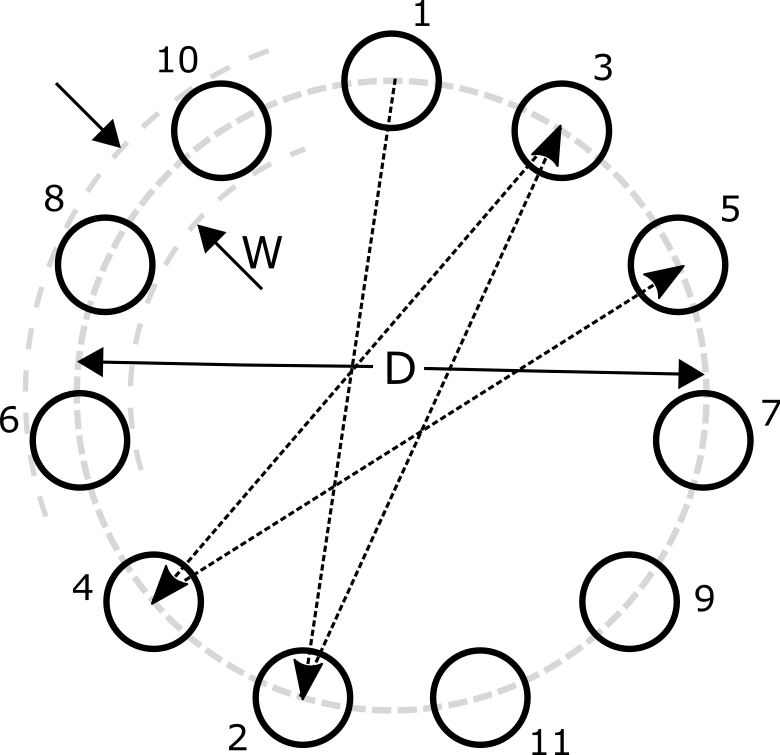
\includegraphics[width=\textwidth]{fitts_circle.png}
    \caption{Fitts' Circle diagram. $D$ is the distance between targets and $W$ is the width of the targets.}
    \label{fig:ph_fitts_circle}
\end{figure}

In this work, we use the effective width for the targets, which is defined as:
\begin{equation}
    W_e = 4.133\sigma
\end{equation}
where $\sigma$ is the standard deviation of the end point positions.
This is known as the adjustment for accuracy\cite{welford_fundamentals_1968}.
This correction accounts for the performance of the subject, especially on lower index of difficulty conditions where they may aim for the inside edge of a target.
Hence, the use of the effective width provides the index of difficulty for the task that the subject performed, not the task presented to them.
The effective width is calculated per subject per distance and width configuration, and subsequently used in the index of difficulty equation.
\begin{equation}
    {ID}_e=\log_2\left(\frac{D}{W_e}+1\right)
\end{equation}

Fitts' Law has been used in evaluating virtual environments and their input devices.
Most of the work has been focused on 3D stereo displays\cite{liu_comparing_2009} or .
Chun et al. (2004) evaluated a set of 3D stereo displays with a single haptic-enabled stylus using a Fitts’ tapping task.
They did not have well-fit regressions, but this could have been due to a small range of ID values used (2-3), targets being placed in 3D space (a 3D task with 3D movement) with random order, and averaging across subjects before completing the regression.
%Teather & Stuerzlinger (2011) performed a similar task and also found an underperformance of the regression in the fully 3D task.
One condition performed a mid-air 2D planar task with 3D movement, and no significant difference in throughput was found compared to the same task with constrained 2D motion.
%Liu et al. (Liu, Van Liere, Nieuwenhuizen, & Martens, 2009) performed a planar multi-directional Fitts’ task with a stereoscopic display, and compared virtual world to real world results, finding movement time twice as long in the virtual condition.
The trajectories were analyzed to determine where the extra movement time was spent, which is discussed in a later section (Trajectories in Virtual Environments).

The use of Fitts' Law with haptics has mostly focused on active haptics\cite{chun_evaluating_2004}.
\rule{0.75\textwidth}{1pt}
\begin{itemize}
  \item fitts law with haptics
  \item collect references
\end{itemize}

\subsection{Presence}

The feeling of presence is often specified as a goal of a virtual environment.
A definition from Witmer and Singer\cite{witmer_measuring_1998} reads:
\begin{displayquote}
\textit{Presence} is defined as the subjective experience of being in one place or environment, even when one is physically situated in another.
\end{displayquote}
Increased presence can lead to increased performance in a virtual environment task\cite{youngblut_relationship_2003}.

\subsection{Arm Fatigue}

Despite the concern of arm fatigue in virtual environments\cite{burdea_virtual_2003}, it was surprising that most results in literature were anecdotal or for mitigations without quantification of the fatigue.
Since fatigue is a subjective quantity, it can be hard to measure it between subjects, and sometimes even within.
The negative impact of arm fatigue on using virtual environments makes it worth investigating.
The arm fatigue scale used within this experiment is a Borg Rating of Perceived Exertion (RPE) scale that ranges from 6-20\cite{borg_borgs_1998}.
Hincapie-Ramos et al.\cite{hincapie-ramos_consumed_2014} proposed a model for quantifying and predicting the amount of arm fatigue that correlated well with a Borg scale.

\section{Methods}

The purpose of the experiment described within this paper is to answer the following research questions:

\begin{enumerate}
    \item Will the throughput be higher with passive haptics?
    \item Do subjects learn the task quicker with passive haptics?
    \item What are the differences between the formation of reaching motion trajectories with passive haptics?
    \item Does the use of passive haptics lower arm fatigue?
    \item Does the use of passive haptics cause greater presence?
\end{enumerate}

\subsection{Experimental Setup}

For the experimental setup, subjects were seated at a desk with a blank panel mounted on an angle in front of them.
The plywood panel (45cm x 45cm) was used to provide only the backstop of the virtual buttons for the ``Passive Haptics'' condition.
The button selection is registered by the subject moving their index finger into a hover zone (cylinder for the circle buttons) in front of the button that extends outward 0.5in.
Their entrance into the hover zone is indicated to them by the button changing color.
A successful button press is registered after 150ms, and is indicated by the color turning off and a button click noise being played over speakers.

The equipment used consists of an Oculus Rift DK2 (Development Kit 2) head-mounted display (HMD) and a LeapMotion hand tracker.
The low-persistence OLED display has a resolution of 1920x1080, with a referesh rate of 75Hz.
The field of view is approximately 100$^\circ$.
It utilizes internal trackers and an external infrared camera for head tracking.

The LeapMotion is a markerless hand tracker which utilizes dual infrared cameras to provide a skelatal level position of hands and fingers in view.
This position is used to provide an image of the hand position in the virtual environment, as well as for determining when a button is pressed.
Instead of using the LeapMotion in its original face-up configuration, it was mounted above the working area and pointed down.
Our pilot studies indicated that hand tracking from the LeapMotion was improved utilizing this face-down setup with the software using the head mounted configuration.
However, the hand tracker could not be mounted on the head mounted display as it required a fixed position relative to the passive haptics to maintain appropriate registration between the virtual world and the passive haptics.

A custom calibration scheme was developed for the hand tracker as the initial registration between physical and virtual worlds was not very accurate.
Despite the inaccuracy, the LeapMotion software was very precise, so after performing the calibration the registration was kept stable.
The calibration performed a least squares claculation to solve for a transformation matrix between known real world locations and the reported location from the LeapMotion.

\subsection{Experimental Task}

The experimental task was a Fitts' circle in the virtual environment, performed by subjects in two haptic conditions.
The subjects were seated at a desk for the experimental task, and the circle was located on a panel mounted on the desk.
The two haptic conditions were ``No Haptics (NH)'' and ``Passive Haptics (PH).''
These conditions are pictured in Figure \ref{fig:ph_conditions}.
For the ``Passive Haptics'' condition a physical panel was co-located with the panel in the virtual world, which was removed for the ``No Haptics'' condition.

\begin{figure}
    \centering
    \begin{subfigure}[t]{0.32\linewidth}
        \centering
        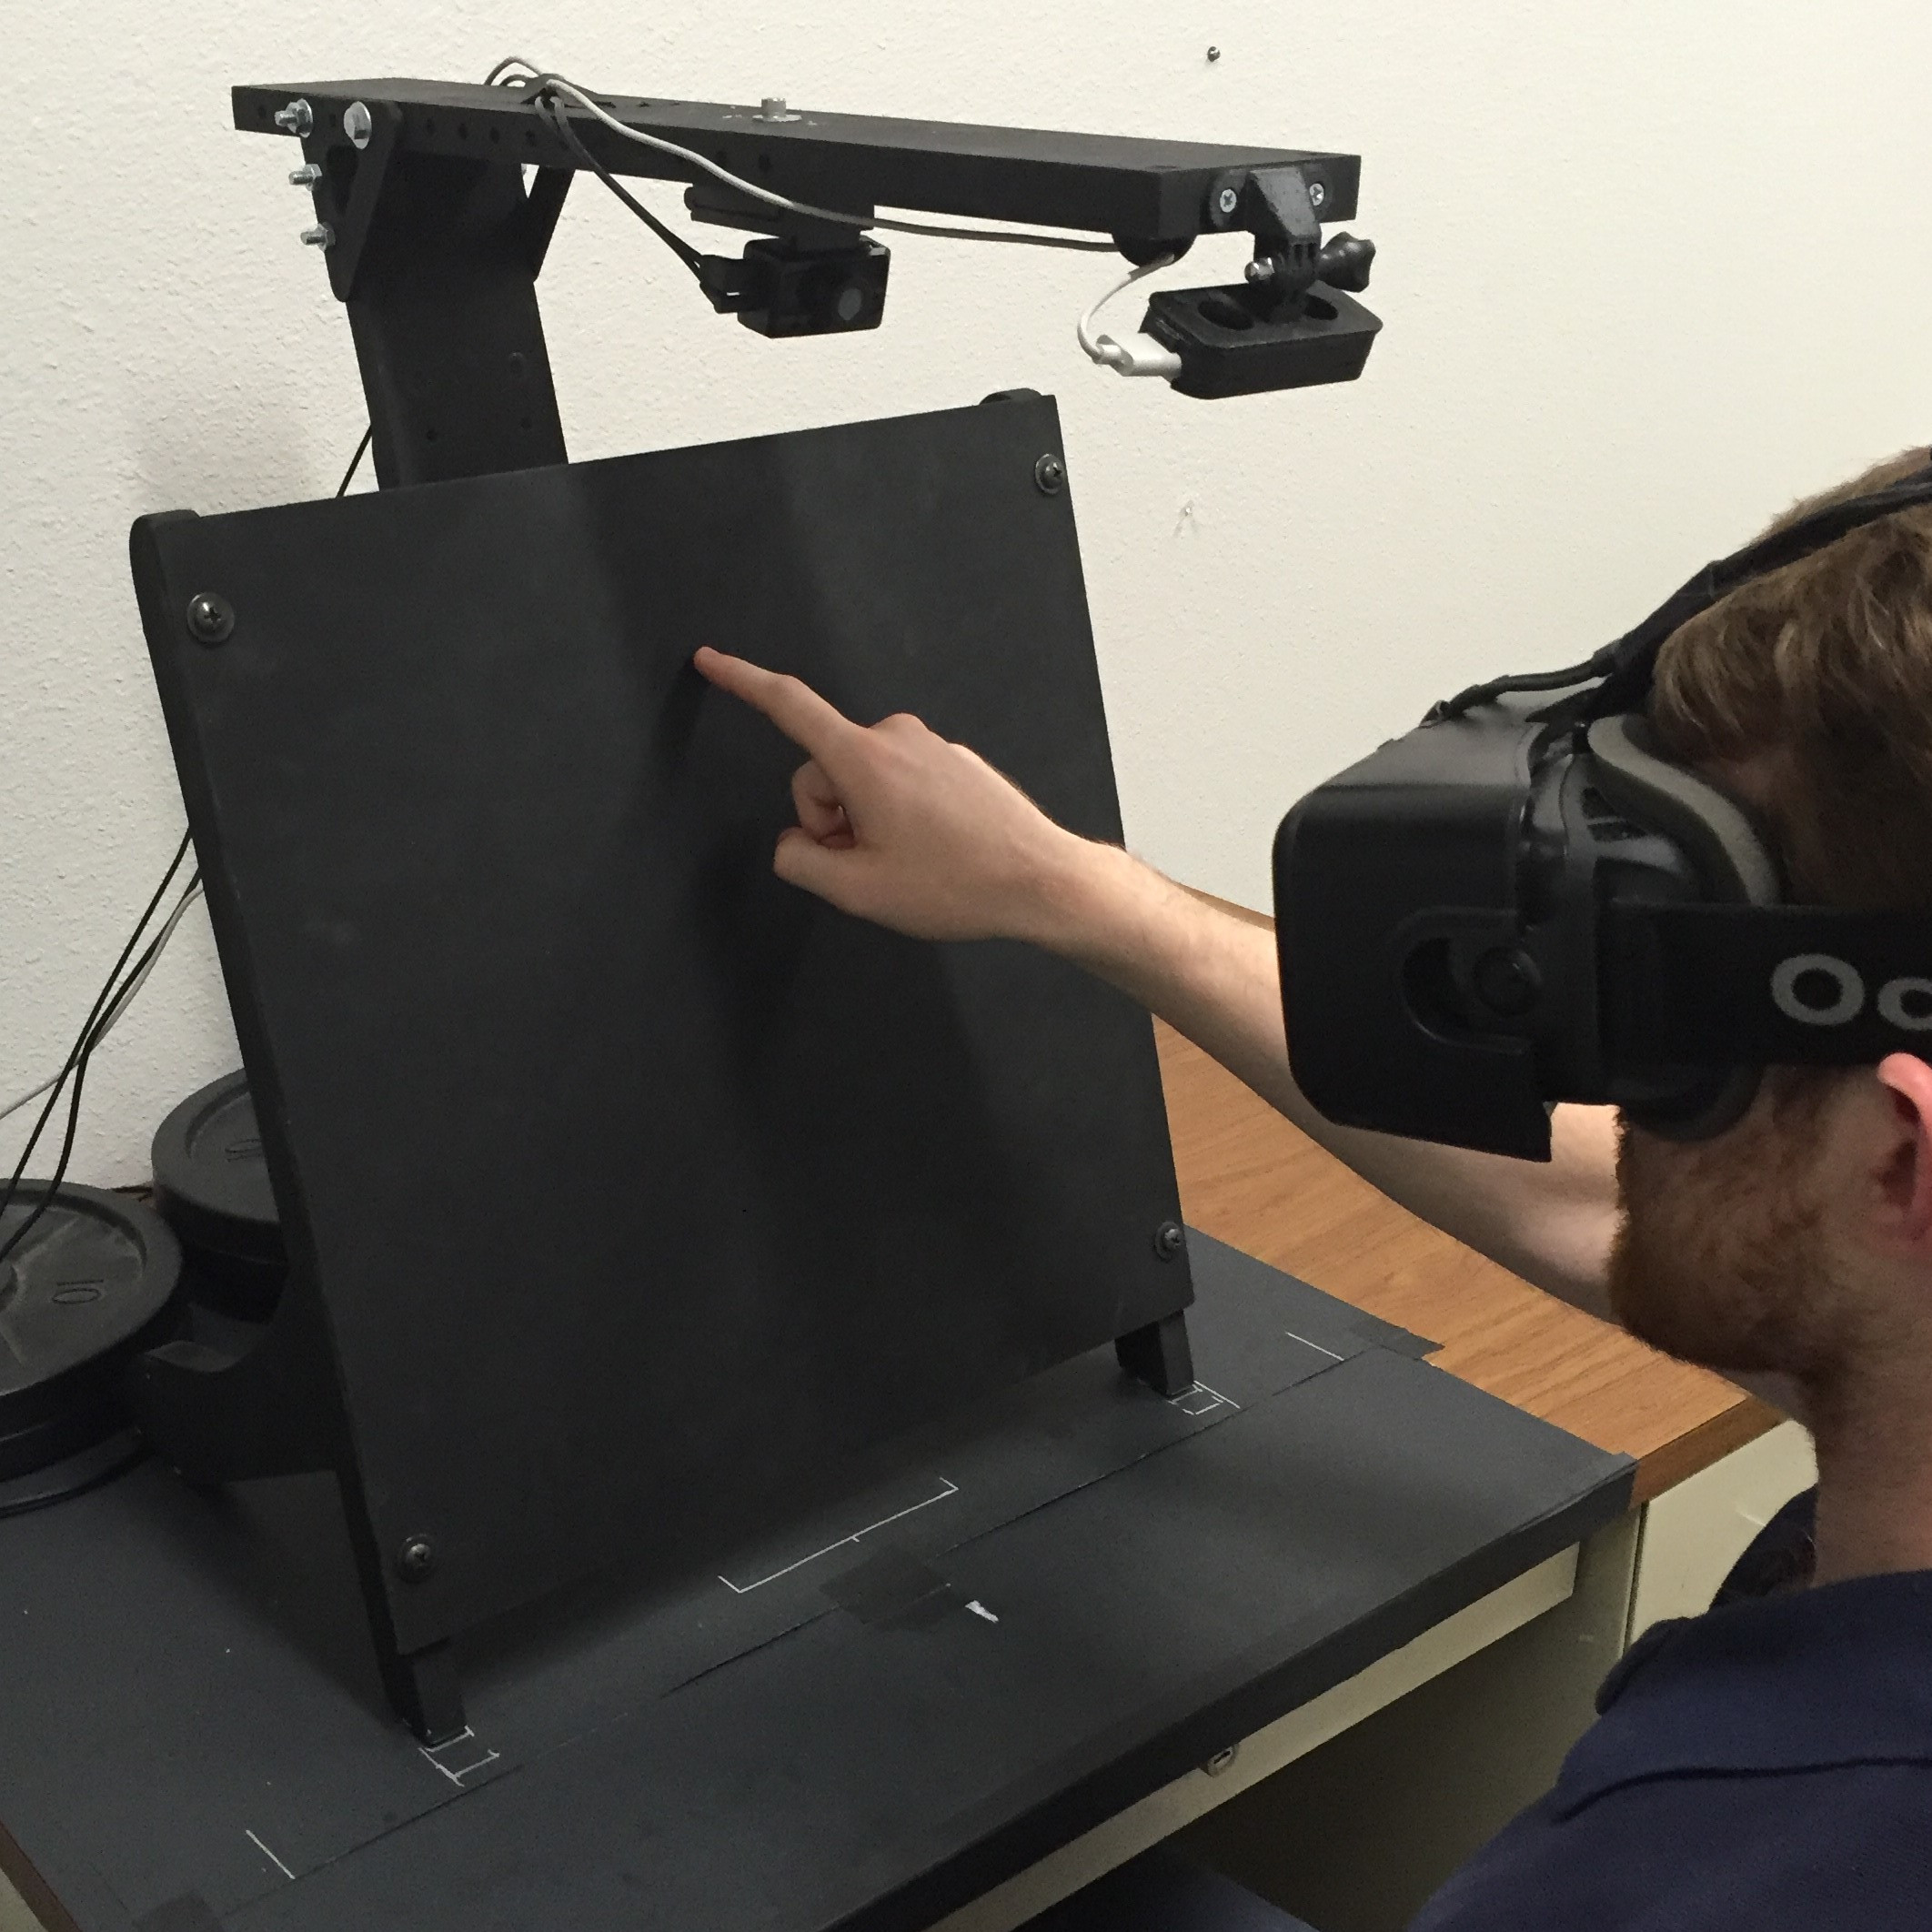
\includegraphics[width=\linewidth]{ph_ph_condition.jpg}
        \caption{Passive Haptics condition}
        \label{fig:ph_conditions:ph_condition}
    \end{subfigure}
    \begin{subfigure}[t]{0.32\linewidth}
        \centering
        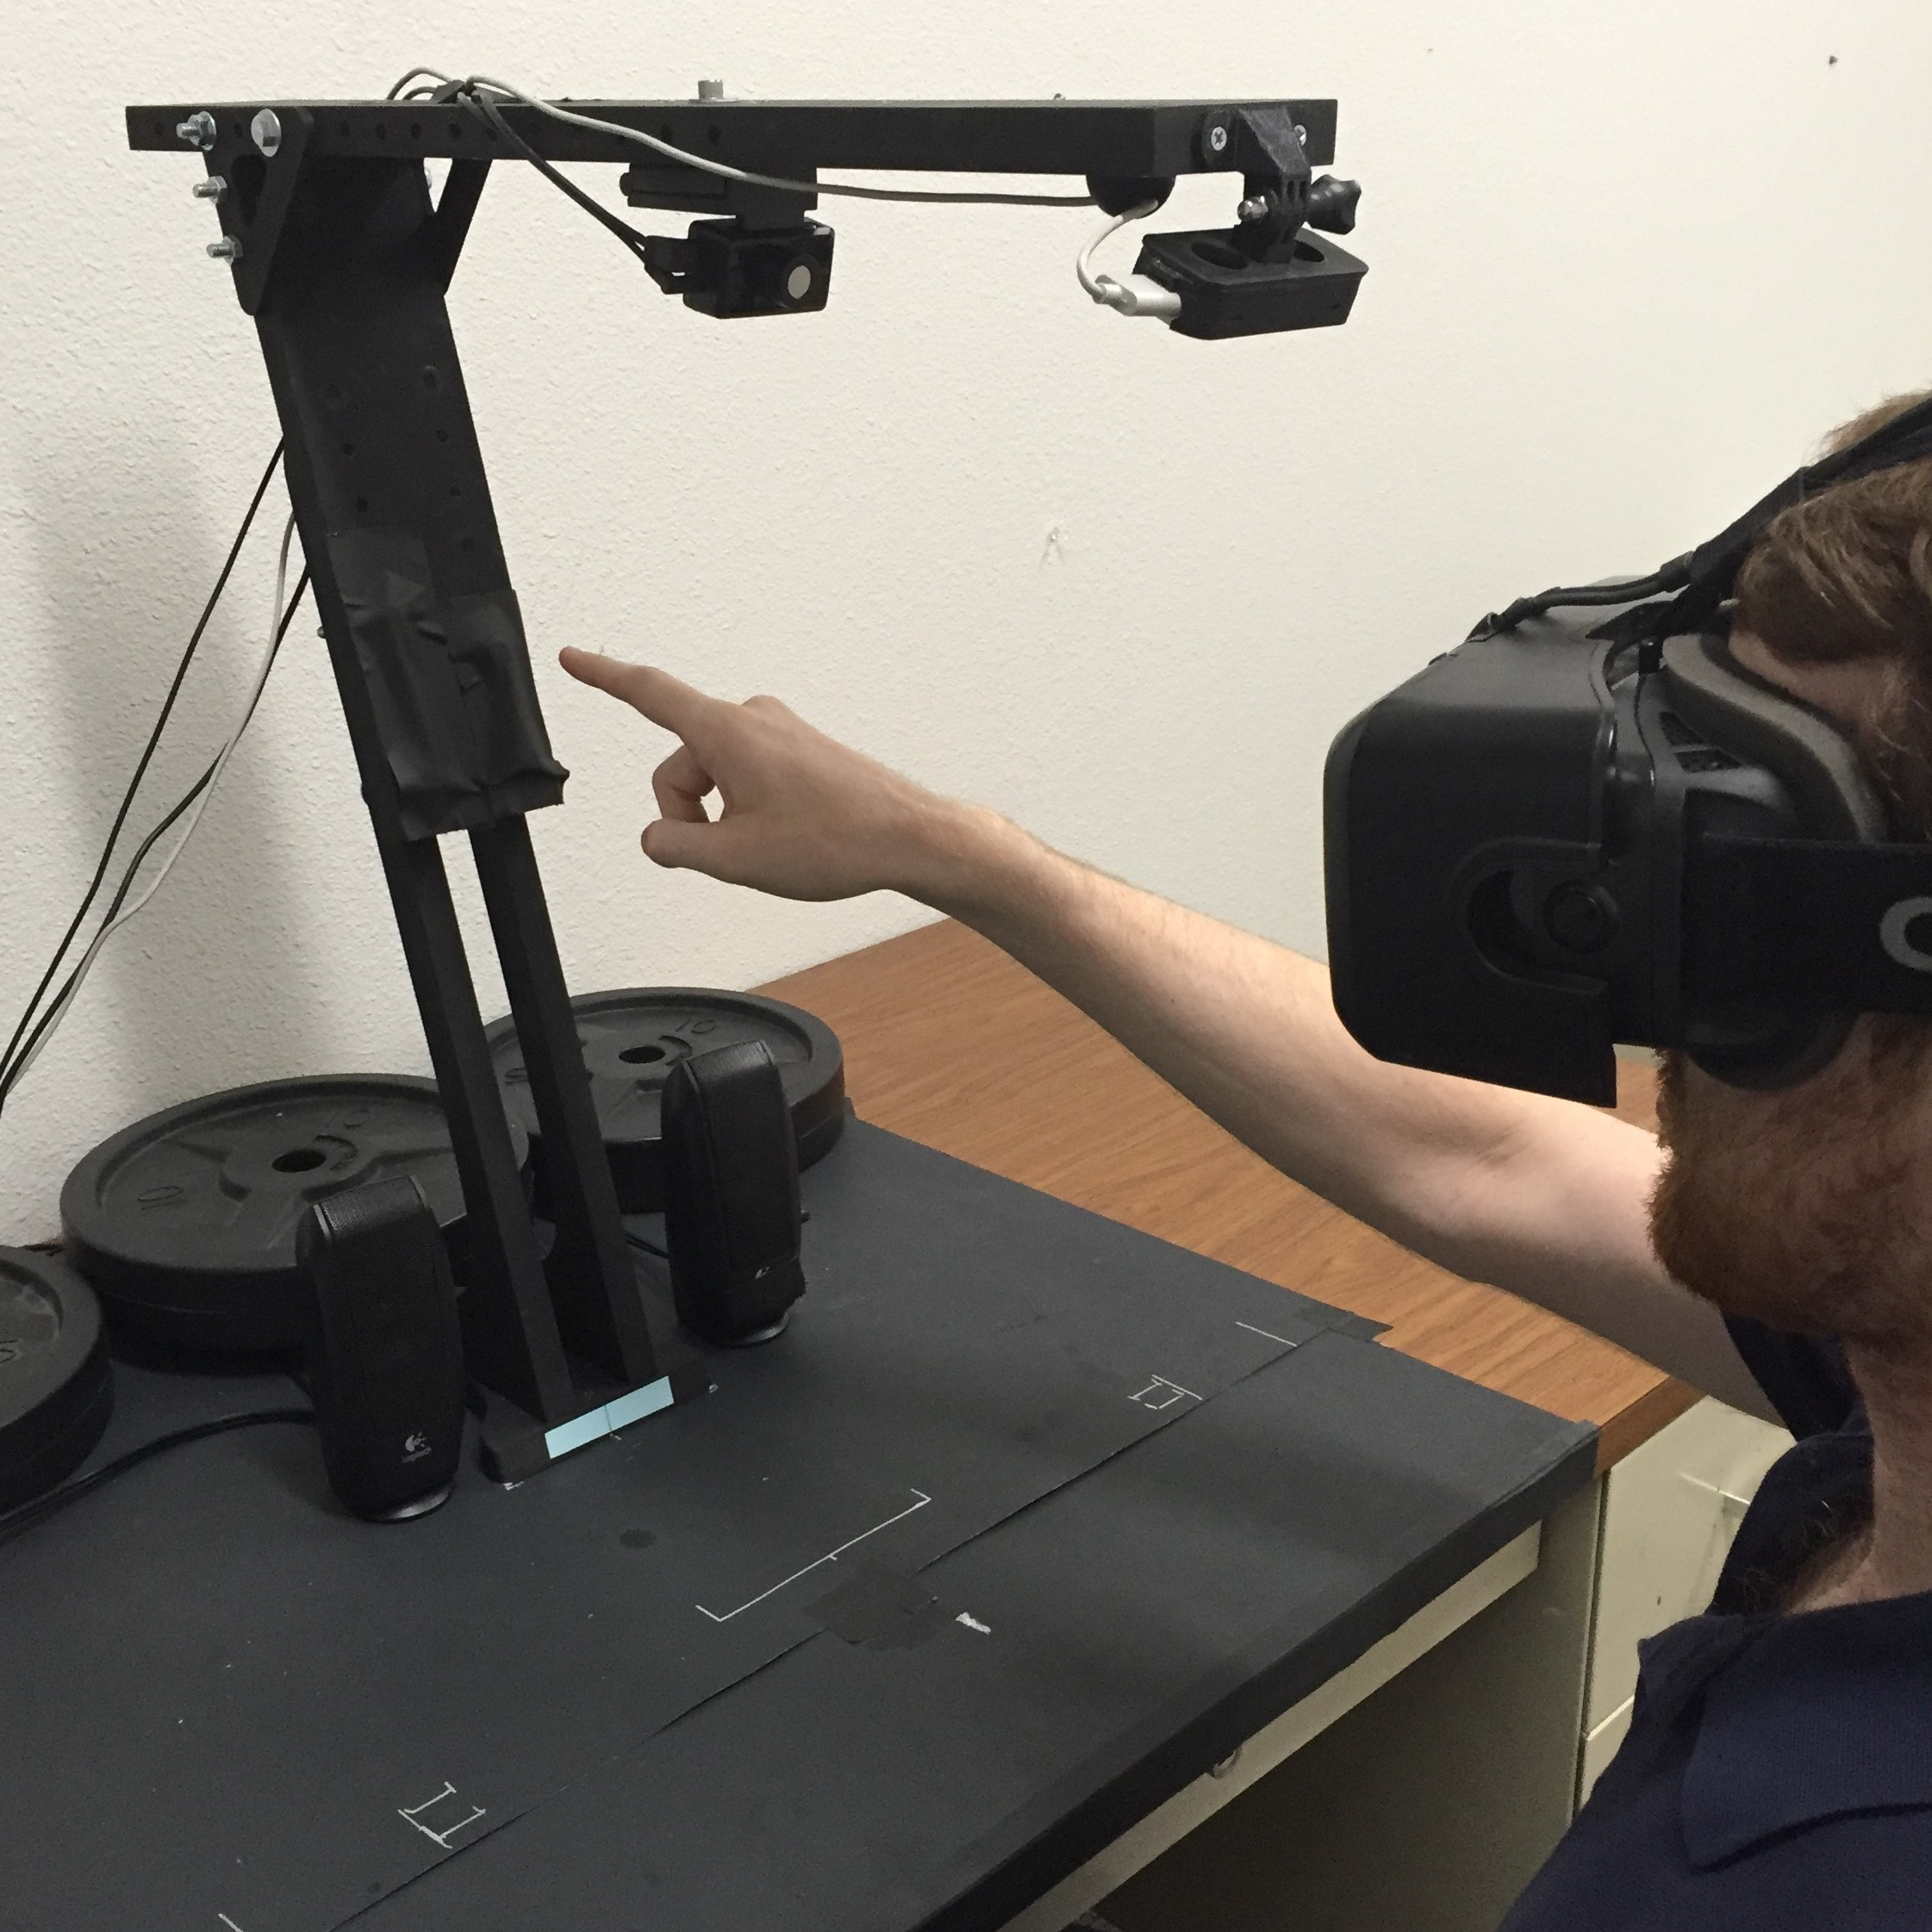
\includegraphics[width=\linewidth]{ph_nh_condition.jpg}
        \caption{No Haptics condition}
        \label{fig:ph_conditions:nh_condition}
    \end{subfigure}
    \begin{subfigure}[t]{0.32\linewidth}
        \centering
        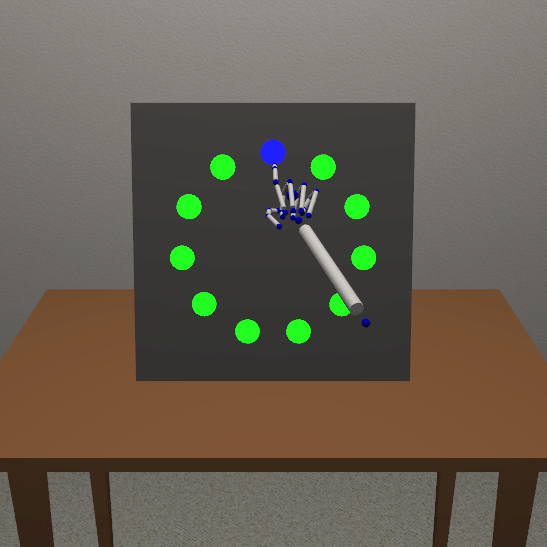
\includegraphics[width=\linewidth]{ph_virtualview.png}
        \caption{View of virtual world}
        \label{fig:ph_conditions:virtual}
    \end{subfigure}
    \caption{Experimental conditions and view of virtual environment.}
    \label{fig:ph_conditions}
\end{figure}

There were no differences to the task itself or the method of button activation.
The only difference between the conditions was the removal of the physical panel.
The hand tracker remained in the same location, preserving the location of the buttons in the virtual environment.
The dimensions of the virtual world were no different for either condition.
In fact, there was no change to the software between the conditions.

Subjects performed the Fitts' circle for three different distances (20cm, 30cm, 40cm) and five different button widths (5mm, 10mm, 15mm, 20mm, and 25mm).
These configurations were chosen to span a wide range of indices of difficulty (3.2---6.4).
For each configuration of distance and width, subjects had to complete the full pattern of 11 buttons three times consecutively.
This set of 33 movements for a single configuration is referred to as a single trial for a subject.
The distance was kept constant for the consecutive trial until all five button widths were complete.
The distances were presented in either smallest to largest or vice versa, which was counterbalanced among subjects.

This set of 15 trials was repeated for each haptics condition and the order was kept the same within subjects.
The sequence that the two conditions were presented to each subject was also counterbalanced.

\subsection{Experimental Design}

As described in the previous section, the experiment was performed with a within-subjects design.
Subjects were asked to complete the same experimental task for both conditions of haptics: Passive Haptics (PH) and No Haptics (NH).
The two different haptic conditions are the main independent variables.

It was expected we would find a large amount of skill transfer between the two conditions, so the order in which subjects performed the two conditions was counterbalanced.
This created a second independent variable that is between subjects.
The subjects who performed the conditions with the PH being their first condition were one group, and the subjects who performed NH as their first condition were a second group.
We call this grouping ``sequence'' and refer to the two groups as ``PH First'' and ``NH First''.

For a Fitts' Law evaluation, it is often recommended that the data collection only begins when the subject is fully trained on the task.
However, one of the goals of the experiment is to investigate the learning rate of the subjects.
For that reason, the subjects were given no seperate training time for the task or virtual environment.

In lieu of collecting the data from fully trained subjects, the throughput analysis will be carried out on movements that are determined to be composed of mostly ballistic motion.
The filtering parameters were determined post-hoc from the trajectory recordings.
Their development and parameter selection are discussed in the Results section.

\subsection{Dependent Measures}

The main dependent measure is the Fitts' throughput, measured through the movement time between button presses.
Additionally, the trajectory of each movement is recorded from the hand tracker for analysis.
To determine the arm fatigue, subjects were asked to rate their arm fatigue on the Borg scale from 6 to 20.
The scale was presented with anchors as shown in Table \ref{tab:ph_borg_scale}.
The arm fatigue rating was collected at the beginning of each condition, and then after every other configuration of distance and width combination (and after the final trial, due to an odd number of trials).
At the completion of each condition the subject was given a presence questionnaire.
At the end of the experiment, an additional condition comparison survey was given to ask for opinions on the two haptic conditions.

\subsection{Trajectory Phases}
\label{sec:ph_traj_phases}

Human reaching movements have long been known to consist of two distinct phases\cite{woodworth_accuracy_1899}.
To seperate the trajectories into the various phases, a simple algorithm was developed.
First, the local minima are found throughout the velocity profile of the movement to seperate the movement into various submovements.
The ``ballistic phase'' is then classified as the submovement which contains the peak velocity of the entire movement.
The various submovements after the ballistic phase are classified as the ``corrective phase''.
Any movement before the ballistic phase is classified as a ``reaction time''.
An example of the results of this classification is shown in Figure \ref{fig:ph_trajectory_ballistic}.
This mathematical definition does break down for certain cases where a subject might have two submovements in the ballistic phase due to a mid-course correction or similar, however one of the main purposes of this classification was to find movements which are appropriate to use for the Fitts' Law calculations.

\begin{figure}
    \centering
    \includegraphics[width=4.0in]{{trajectory_velocity.ballistic}.png}
    \caption{Example trajectory with three phases indicated.}
    \label{fig:ph_trajectory_ballistic}
\end{figure}

\subsection{Trajectory Filtering}

We used a low-pass filter on the trajectory recordings to reduce the amount of noise.
The LeapMotion processes data at a variable frequency, thus creating a variable rate for recording.
The frequency typically varies from about 100Hz to 120Hz.
To perform the filtering, the data was first resampled to a fixed rate of 100Hz.
The filter used is a fourth-order Butterworth filter with a cut-off frequency of 5Hz.
The cut-off frequency was chosen as voluntary hand movements have been shown to be below such a rate\todo{citation needed}.

\subsection{Statistical Methods}

The throughput, arm fatigue rating and presence score were all statistically tested using a two-way ANOVA with one within-subjects factor (Haptics) and one between subjects factor (Sequence).
When the ANOVA showed an interaction effect, the two Sequence groups were seperated and a repeated measures t-test was performed for the Haptics factor with each group.
The statisitical significance level was corrected using the Bonferroni correction given the three dependent measures being tested.
This leads to effects being considered statistically significant at the 0.0167 level ($\alpha=0.05/3=0.167$).
Effects between $0.05 < p < 0.0167$ are noted as marginally significant.
Additionally, the presence questionnaire was tested using Cronbach's alpha for internal consistency.

\section{Results}

\subsection{Participants}

Twenty (20) subjects were recruited from the UC Davis engineering student population, both undergraduate and graduate students.
The age range was 19---29 ($M=22.95, \sigma=3.0$) with 16 males and 4 females.
The genders were balanced amongst the counterbalanced groups.
All subjects indicated either less than one hour or no prior experience with virtual reality.

\subsection{Throughput}

The throughput is calculated per movement using Equation \ref{eq:throughput} and meaned per trial before being meaned per subject and condition.
Throughput is used to investigate the first two research questions: do the subjects learn quicker and does their throughput performance improve with passive haptics.

\subsubsection{Rate of Learning}

\begin{figure}
    \centering
    \includegraphics[width=\textwidth]{{throughput_trials.8.0x4.0}.png}
    \caption{Throughput per trial. The learning curve exponential fit is given by Eqn. \ref{eq:ph_learning} with parameters from Table \ref{tab:ph_tp_regression}.}
    \label{fig:ph_throughput_trials}
\end{figure}

The average throughput for each trial, seperated by haptics condition, is shown in Figure \ref{fig:ph_throughput_trials}.
An exponential rise to a learned state can be fit to each haptics condition to model the learning curve of the subjects.
The equation used is given as:
\begin{equation}
    \mathrm{TP}(T) = \mathrm{TP}_{\infty} - (\mathrm{TP}_{\infty}-\mathrm{TP}_0)e^{\left( -T / \tau \right)}
    \label{eq:ph_learning}
\end{equation}
where $T$ is the trial number, $\mathrm{TP}_{\infty}$ is the asymptotic learned value of throughput, $\mathrm{TP}_0$ is the initial value at $T=0$ and $\tau$ is the time constant.
The time constant is the amount of trials for the throughput to rise 36\% of the difference between the fully learned throughput ($\mathrm{TP}_{\infty}$) and the initial throughput ($\mathrm{TP}_0$).
The parameters of the fit for each condition is shown in Table \ref{tab:ph_tp_regression}, as well as the standard error of the estimate (SEE).
The value of throughput from the regression fit as a percentage of $\mathrm{TP}_{\infty}$ for certain trials are listed in Table \ref{tab:ph_tp_regression_values}.

The rate of learning is very similar amongst both groups in the first condition.
For the first condition it can appear that the subjects performing NH learned quicker than their counterparts performing PH by looking at the time constants.
However, as the values in Table \ref{tab:ph_tp_regression_values} show, the NH First group started their first trial at a lower percentage of their learned state.
The shape of the learning curves are very similar and both groups reached approximately 90\% of their fully learned state by the 5\textsuperscript{th} trial.

The learning curves are quite different for the second condition.
The NH condition does not have a learning curve, with a straight line being a better fit than the exponential function.
This indicates the transfer of training from the PH condition allowed the group who did PH first to immediately perform in NH at the same level as the fully learned state of the subjects who learned NH in their first condition.
This transfer of training to the second condition did not occur as strongly for the group who did NH first.
Their initial performance of PH did start out at a slightly higher level than the subjects who did PH first (2.8 bps vs 2.4 bps), but after 5 trials this difference had converged (3.6 bps vs 3.7 bps).

\begin{table}
    \centering
    \includetable{throughput_regressions.tex}
    \caption{Exponential fit parameters of Eqn. \ref{eq:ph_learning}. Curves are shown in Figure \ref{fig:ph_throughput_trials}.}
    \label{tab:ph_tp_regression}
\end{table}

\begin{table}
    \centering
    \includetable{throughput_regression_values.tex}
    \caption{Percentage of fully learned state for various trials for each group and condition. $\mathrm{TP_i}$ is $\mathrm{TP}(i)/\mathrm{TP}_{\infty}$ using Eqn. \ref{eq:ph_learning}.}
    \label{tab:ph_tp_regression_values}
\end{table}

These results indicate that subjects did not learn faster with Passive Haptics.
The only differences between learning rates is the positive transfer of training from performing Passive Haptics first and No Haptics second.
The answer to the research question \textit{Do subjects learn the task quicker with passive haptics?} appears to be that the passive haptics does not make subjects learn faster, but they are able to learn the task quicker without passive haptics afterward.
It does appear that the fully learned state is different between the haptic conditions, which is investigated further in the next sections.

\subsubsection{Ballistic Movement Filtering}
\label{sec:ph_ballistic_filter}

Before they could be used for the Fitts' Law analysis the trajectories were filtered so that only movements which were direct to target were included.
A well-learned movement appropriate for Fitts' Law is one which moves directly towards the target and does not have much extranous movement or idle time beyond what is required to complete the task.
A number of deviations from these well learned movements were observed in the dataset which we aimed to filter out for the final throughput calculations.
We describe in this section the three metrics developed that were used to determine whether a movement was direct to target.

%An inordinate amount of time was spent either in the reaction phase before the ballistic, or more typically, after the ballistic movement in the corrective phase.
%There were two common causes of a long time spent in the corrective phase, the first was that the subject had trouble finding the activation zone or holding it there for the 160 msec required.
%The second cause was that the subject would have a false start and move towards the next target before their button press was activated.
%For the former, this led to a increase in time for the corrective phase, but not neccesarily a large path distance increase.

%To perform the filtering, three metrics were developed.
The first metric was the ratio of path distance travelled in the ballistic phase to the distance between the targets for that movement (i.e. 20cm, 30cm or 40cm).
Ideally, the ballistic portion would cover the majority of the distance between the targets.
A movement which covered too little of the target distance could mean the subject slowed or stopped in the middle of movement, and one that covered more could mean the subject overshot or had an indirect trajectory.
A sample movement that gets flagged by this filter is shown in Figure \ref{fig:ph_traj_filter_target}, which has a ratio of 1.49.
This is an example of a movement that does seemingly have a direct movement toward the target, but includes a large deviation perpindicular to the movement axis.
This deviation could mean the subject initially aimed their ballistic portion in the wrong direction but performed a correction during the movement.
The limits for this filter were chosen as having a ratio between 0.90 and 1.10, i.e.\ within 10\% of the target distance.
This filtered out 4577 of the 17970 movements.

\begin{figure}
    \centering
    \includegraphics[width=4.0in]{{trajectory_both.bad_target_filter}.png}
    \caption{An example of a movement with a large ballistic distance to target distance ratio. The bottom plot shows the projection of the trajectory on the plane of the Fitts' circle.}
    \label{fig:ph_traj_filter_target}
\end{figure}

The second filtering metric was also based on the ballistic phase path distance.
For this metric it was compared to the total path distance the subject travelled for their entire movement.
This filter targetted movements where after the ballistic phase the subject moved away from the target, or had a smaller but significant movement before the main ballistic movement.
An example is shown in Figure \ref{fig:ph_traj_filter_distance} which shows a movement which passed the first metric (the ballistic phase distance ratio to the target distance was 1.03), but the ballistic phase was only 56\% of the total distance travelled during that movement.
This was a common problem where a subject would have a false start and move towards the next target before their button press was activated.
The threshold was set at 0.80 which has 4264 movements lower than the threshold, though only 1675 were unique from the target distance filter.

\begin{figure}
    \centering
    \includegraphics[width=4.0in]{{trajectory_both.bad_distance_filter}.png}
    \caption{An example of a movement with a small ballistic distance to total path distance ratio. The bottom plot shows the projection of the trajectory on the plane of the Fitts' circle.}
    \label{fig:ph_traj_filter_distance}
\end{figure}


The last filter took a time based approach, and looked a the ratio of the time spent in the ballistic phase over the total movement time.
This filter removed movements where the subject spent an inordinate amount of time either before or after the ballistic phase.
If they were not moving during the non-ballistic phases, it would not have been caught by the distance-based filters either.
The threshold of 0.40 meant that 4496 movements were filtered, however only 873 of those are unique of the other two filters.
Figure \ref{fig:ph_traj_filter_time} illustrates a movement where the subject waited before initiating the ballistic movement.
Since the subject did not move during this idle time, the other two filters did not flag this movement.

\begin{figure}
    \centering
    \includegraphics[width=4.0in]{{trajectory_both.bad_time_filter}.png}
    \caption{An example of a movement with a small ballistic time to total time ratio. The bottom plot shows the projection of the trajectory on the plane of the Fitts' circle.}
    \label{fig:ph_traj_filter_time}
\end{figure}

The combination of these three filters led to 7125 of 18000 movements being filtered out, leaving 60\% of the movements.
For each of the metrics, the threshold was determined by investigating the distribution and looking at sample movements on either end of the threshold to determine if it was an approriate value.

The final check before performing the Fitts' calculation was to ensure that each trial had enough data for the adjustment for accuracy calculation.
The adjustment for accuracy is based on the distribution of endpoint data from a single trial (which is one distance and width configuration).
One trial consists of 30 consectutive movements, but the ballistic filtering could diminish the amount remaining in each, so a trial was only included if at least half (15 of 30) movements were considered to be good movements by the ballistic filters.
This means that movements from a trial that did not have enough good movements were also filtered out from the Fitts' calculation.
Not only is this important to make sure the adjusted width is valid, it also removes trials where the subject likely did not reach a fully learned state, as most of their movements were not primarily ballistic movements direct to target.
On average, 11 of 15 trials per condition from each subject ($M=10.98, \sigma=3.25$) had enough good movements to be included.
This left 9218 movements for the Fitts' calculation, just over half of the total movements (51.3\%).
Slightly more movements were filtered from the No Haptics condition, with 47.1\% of NH movements left after the filtering, compared to 55.5\% of the PH movements.

\subsubsection{Throughput}

The throughput was found to be higher in the PH condition, at 4.25 bps compared to the 3.76 bps of the NH condition.
A two-way mixed ANOVA was performed to determine the effect of haptics condition.
Since we already expected order effects and have seen them with the transfer of training seen in the Rate of Learning section, the sequence the subjects performed the haptic conditions was a between subjects factor.
The effect of haptics was found to have a significant effect on the throughput ($F(1,18)=35.59, p<0.001$) between the PH condition ($M=4.25, \sigma=0.44$) and the NH condition ($M=3.76, \sigma=0.38$).
There was no effect on throughput based solely on sequence group ($F(1,18)=0.53, p=0.47$), but there was a marginally significant interaction effect between the sequence and haptics ($F=(1,18)=4.48, p=0.048$).

As can be seen in Figure \ref{fig:ph_throughput}, this marginal interaction effect appears to indicate that both groups had improved performance but the PH First group performed better at the NH condition.
The post-hoc repeated measures ttest between haptic conditions for the subjects who performed PH First was significant ($t(9)=4.62, p<0.001$), with the PH condition ($M=4.23, \sigma=0.34$) outperforming the NH condition ($M=3.91, \sigma=0.40$).
The mean of the differences between subjects was 0.32 bps.
The group of subjects who performed NH first also had a significant effect ($t(9)=3.96, p<0.001$) the PH condition ($M=4.28, \sigma=0.54$) and the NH condition ($M=3.62, \sigma=0.32$), with a higher mean of differences of 0.66 bps.
These post-hoc tests confirm that both groups had a significant effect of haptics, though the NH First group had a larger difference between the conditions.

\begin{figure}
    \centering
    \includegraphics{{throughput.4.0x4.0}.png}
    \caption{Throughput boxplot by haptics and sequence.}
    \label{fig:ph_throughput}
\end{figure}

It is worth noting that without using the ballistic filter, the major conclusions found do not change.
The only major difference is the magnitude of the throughput and size of the differences.
The statistical tests have the same results as well.
The results by haptics for both filtered and unfiltered are shown in Table \ref{tab:ph_throughput_fulltable}.
These results indicate that subjects do have higher throughput with passive haptics, answering our first research question.

\begin{table}
    \centering
    \includetable{throughput_fulltable.tex}
    \caption{Throughput scores by haptics condition.}
    \label{tab:ph_throughput_fulltable}
\end{table}

% Factors causing this.

% Counts of the filters

\subsection{Trajectory Phases}

As described in Section \ref{sec:ph_traj_phases}, each movement of the subjects can be dissected into three distinct phases: reaction time, ballistic phase, and corrective phase.
We have already seen that, overall, the subjects took more time to complete a movement without the passive haptics in place with the results of throughput.
In this section we investigate the differences in time spent in the three phases.
We report here the means of time spent in each of the three phases.
Times reported are all milliseconds.
The results also include the filtered and unfiltered results, where the filtered results only include movements that were deemed purely ballistic by the filtering methods in Section \ref{sec:ph_ballistic_filter}.
The unfiltered results include all movements.
The phases were meaned per subject first, and then by condition.
The time spent in each phase is listed in Table \ref{tab:ph_phases}.
Each phase was tested for the effect of haptics and sequence through a mixed two-way ANOVA.

The reaction time had no effect by haptics ($F(1,18)=0.32, p=0.58$) or sequence ($F(1,18)=0.001, p=0.98$).
However, for the interaction between the two a significant effect was found ($F(1,18)=18.56, p<0.001$).
The interpretation of this interaction effect without main effect significance is that the first and second condition had a different reaction time, without dependence on the haptics condition or group.
The mean reaction time in the first condition was 130.9 milliseconds ($\sigma=41.0$), but in the second condition it was just over 20 milliseconds faster, with an average of 109.1 milliseconds ($\sigma=36.6$).
The reaction time for both conditions was lower than generally accepted values for reaction time to a visual or aural stimulus\todo{citation needed}.
This is not surprising, as the task was a serial task which the subjects would likely learn the pacing of throughout the experiment.
They would learn to anticipate the activation of a button (which was also the start of the next movement) as it would activate 160 msec after the subject entered the zone of the previous button.
In fact, this interaction effect tells us that subjects did learn how to anticipate the activation event independent of the haptics or the order they performed the seqeunces.
%When including all the movements in the unfiltered case, the reaction time also has no significance due to the effect of haptics or sequence, but it .
%It also does not have a significant interaction effect, which is not surprising as the unfiltered movements were un

The ballistic phase time had a significant effect of haptics ($F(1, 18)=24.14, p<0.001$) between PH ($M=772.6, \sigma=67.7$) and NH ($M=719.5, \sigma=60.0$).
There was no effect of sequence or the interaction effect between haptics and sequence.
Since the ballistic phase should be mostly independent of the use of passive haptics, it was not expected to see the ballistic phase have an effect of haptics.
It is unclear the exact mechanism that led to this, but it could likely be an artifact of the passive haptics causing the subjects to learn the movement, and thus allowing them to move quicker.
There is little difference between the filtered movements and unfiltered movements results, the difference of the means were within a few milliseconds.

The corrective phase time also had a significant effect of haptics ($F(1, 18)=22.46, p<0.001$) between NH ($M=256.6, \sigma=42.1$) and PH ($M=199.1, \sigma=48.1$).
There was no effect of sequence or the interaction effect between haptics and sequence.
This result was expected as one of the main benefits of the passive haptics is that the subject does not have to `find' the target along one dimension.
There was a more noticeable difference between the results of the unfiltered and filtered movements for the corrective phase.
The corrective phase time was much higher in both conditions, with PH having a mean of $564.7$ ($\sigma=253.6$) and NH having a mean of $837.2$ ($\sigma=293.2$).

\begin{table}
    \centering
    \includetable{phases_fulltable.tex}
    \caption{Time in each movement phase by haptics conditions.}
    \label{tab:ph_phases}
\end{table}

\subsection{Arm Fatigue}

The subjects were asked for a rating of their arm fatigue every other trial, as well as before the first trial and after the last trial of each condition.
One trial lasted for 30 movements and consisted of a single distance and width configuration.
The scale ranged from 6 to 20, and subjects were allowed to record decimal ratings.
The full scale with anchors are shown in Appendix \ref{}\tinytodo{where is this}.
The average rating at each trial, seperated by haptics condition, is shown in Figure \ref{fig:ph_armfatigue_trials}.

\begin{figure}
    \centering
    \includegraphics[width=\textwidth]{{armfatigue_trials.8.0x4.0}.png}
    \caption{Arm Fatigue by Trial.}
    \label{fig:ph_armfatigue_trials}
\end{figure}

There is an evident difference between the two haptic conditions for the first condition performed, with the NH condition subjects accumulating more fatigue throughout the trials.
At the end of the first condition, the subjects who performed the PH condition rated their arm fatigue 3.25 points lower on average than the NH condition subjects.
Both groups have a similar rate of recovery, but the second condition quickly converges and shows no apparent difference between the two haptics conditions.

A within-subjects repeated measure (haptics) with two between-subjects measures (sequence and trial) ANOVA was performed to test the significance of haptics and the interaction effect of haptics and sequence.
The interaction effect of haptics of sequence was found to be significant ($F(1, 18)=22.6, p<0.001$) as well as the main effect of haptics ($F(1, 18)=5.47, p=0.03$).
As a result of the significant interaction effect, a post-hoc ANOVA with Haptics and trial as the two within subjects repeated measures was run on both sequence groups.
The NH First group had no effect due to haptics ($F(1, 9)=2.08, p=0.18$), consistent with the observations from Figure \ref{fig:ph_armfatigue_trials}.
The subjects rated the same trial between conditions an average of only 0.69 ($\sigma=2.1$) points higher for the PH condition, which was their second condition.
The PH First group did have a significant effect due to haptics ($F(1, 9)=42.37, p<0.001$).
This group rated the PH condition an average of 2.0 ($\sigma=2.0$) points lower within trials.
As expected, the effect of trial number was significant for all of these tests ($p<0.0001$).

These results show that the subjects only had reduced arm fatigue using the passive haptics for the first condition.
For all other conditions the arm fatigue ratings reached the same level by the end of the condition.
% Why is this

\subsection{Presence}


The presence survey was adminsistered after each haptics condition.
The questions had a 7-point Likert scale response with anchors at either end and the middle.
The score given in this section is a sum of the responses, on a scale of 1 to 7, where a higher score indicates higher presence.
A few questions were asked with an inverted scale (i.e.\ a score of 1 indicated higher presence) and were reversed before the score was calculated.
The internal consistency of the presence questionnaire was tested per condition using Cronbachs' alpha, and was found to be consistent in both conditions ($\alpha=0.72$ and $\alpha=0.71$ for PH and NH, respectively).
The full survey questions and average responses per condition are listed in Table \ref{tab:ph_presence}.
The item total correlation (the correlation between the questions' score and the total score) is also listed for each question.

\begin{table}
    \centering
    \includetable{presence_scores.tex}
    \caption{Presence Score Summary}
    \label{tab:ph_presence_scores}
\end{table}

The average scores per condition are given in Table \ref{tab:ph_presence_scores}.
The presence scores were tested with a mixed within subjects repeated measures (haptics) and between subjects measures (sequence) ANOVA.
The score had a marginally significant effect between Haptics conditions ($F(1,18)=6.08, p=0.024$), with Passive Haptics having a slightly higher mean ($M=77.7, \sigma=9.56$) than No Haptics ($M=71.0, \sigma=9.70$).
There was no significant effect of Sequence ($F(1,18)=4.01, p=0.58$) nor for the interaction effect between Sequence and Haptics ($F(1,18)=0.71, p=0.41$).

\begin{table}
    \centering
    \includetable{ph_presence.tex}
    \caption{Presence questions.}
    \label{tab:ph_presence}
\end{table}

\todo{Discuss results of items.}

\subsection{Condition Comparison}

\begin{table}
    \centering
    \includetable{ph_comparison.tex}
    \caption{Condition comparison survey summary of results.}
    \label{tab:ph_comparison}
\end{table}

The condition comparison survey asked the subjects five questions directly comparing the two conditions.
A summary of their answers are shown in Table \ref{tab:ph_comparison}.
The subjects overwhelmingly responded that they preferred the Passive Haptics (PH) condition (Q5), with all but two subjects choosing it.
In fact, no subject preferred the No Haptics (NH) condition, the two subjects who did not choose PH responded that neither was more preferred.

The other questions had responses similar to the results from the other sections.
The majority of subjects responded that they were more accurate and faster in the PH condition (Q1 and Q2), which agrees with the throughput results.
The subjects who chose Neither or NH were usually not actually faster or more accurate in the NH condition.
In fact, only two subjects had a throughput that was higher in the NH condition, and neither subject chose NH as the condition they performed faster in, though one did say they performed more accurately in the NH condition.

Question 4 asked subjects directly about their feeling of presence, and 13 subjects chose PH, with the remaining split between 4 saying neither and 3 saying NH.
The results of the presence questionnaire suggested that subjects felt more present with the passive haptics, which this agrees with.
The arm fatigue question (Q3) was worded to ask which condition they felt provided more or quicker arm fatigue, and 13 subjects felt this was the case with the NH condition.
The remaining were split between neither (3) and PH (4).
The results of the arm fatigue questionnaire during the experiment found a similar result as the condition comparison survey.

\section{Discussion}

\begin{itemize}
  \item time of each button press
  \item trajectory information for filtering
  \item arm fatigue rating every other circle
  \item presence questionnaire after each condition
  \item condition comparison questionnaire at end of experiment
  \item naive button registration
  \item arm fatigue not validated
\end{itemize}

\section{Conclusion}

